\begin{frame}{Redes Neuronales}
    \textbf{Redes Neuronales}\\
    Las redes neuronales son un subconjunto de machine learning. Están inspirados por el cerebro humano, imitando la forma en que
    las neuronas biológicas se señalan entre sí.
    \begin{figure}[H]
        \centering
        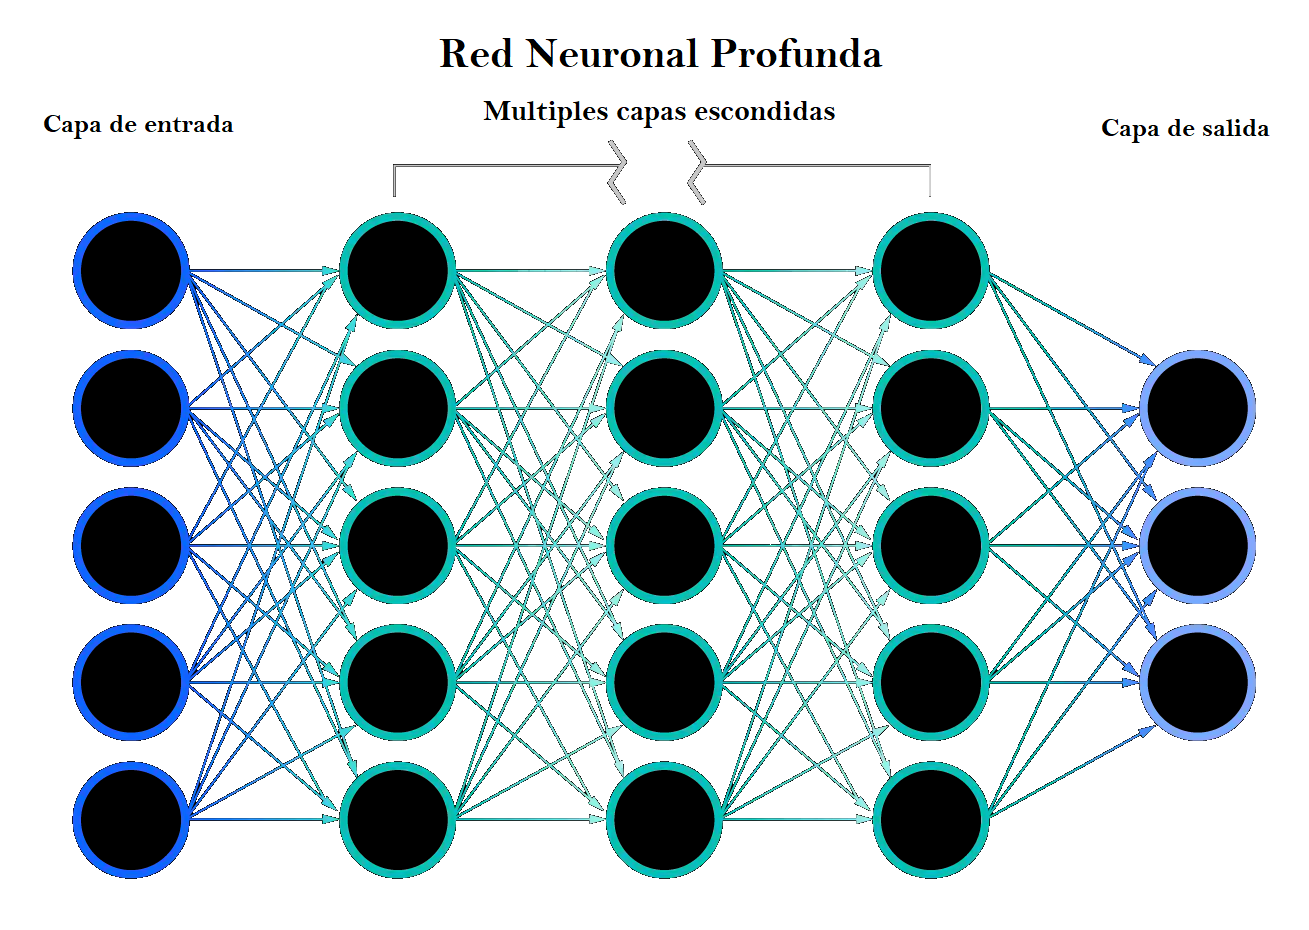
\includegraphics[scale=0.2]{Red_Neuronal.png}
        \caption{Estructura de una red neuronal}
        \label{fig:SRCNN_RedNeuronal}
    \end{figure}
\end{frame}

\begin{frame}{}
    Cada nodo o neurona de la red recibe datos de entrada $x_i$ y realiza la suma mediante ponderaciones $w_i$, además de agregar
    un sesgo $bias$ y finalmente nos da una salida $f(x)$ solo si $f(x)\geq umbral$, de lo contrario la salida será $0$.
    \begin{align}
        \label{eqn:SRCNN_RedNeuronal}
                     x&=\sum_{i=1}^{m}\omega_ix_i+bias
    \end{align}
    \begin{equation}
        \begin{split}
            f(x)\hspace{0.5cm}si\hspace{0.1cm}f(x)\geq umbral \\
            0\hspace{1.0cm}si\hspace{0.1cm}f(x) < umbral
        \end{split}
    \end{equation}
\end{frame}

\begin{frame}{Red Neuronal Convolucional}
    Las Redes neuronales convolucionales son un tipo de redes neuronales artificiales que utilizan la
    convolución para extraer extraer características\\
    \textbf{Convolución}\\
    Consiste en tomar \emph{grupos de pixeles cercanos} de la imagen de entrada e ir operando
    matemáticamente (producto escalar) contra una pequeña matriz que se llama kernel.
    \begin{figure}[H]
        \label{fig:SRCNN_Convolucion}
        \centering
        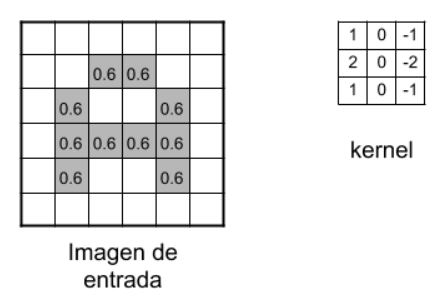
\includegraphics[scale=0.45]{Convolucion.png}
        \caption{Convolución con \textbf{kernel} de $3\times 3$}
    \end{figure}
\end{frame}

\begin{frame}{Descenso del gradiente}
    El \textbf{descenso del gradiente} en conjunto con el algoritmo de \emph{backpropagation} es utilizado para hacer que la red
    \emph{aprenda}.
    \begin{align}
        \label{eqn:SRCNN_DescensoGradiente}
        x_{n+1}=x_n-\alpha\nabla f(x_n)
    \end{align}
    \begin{figure}[H]
        \label{fig:SRCNN_GradDescent}
        \centering
        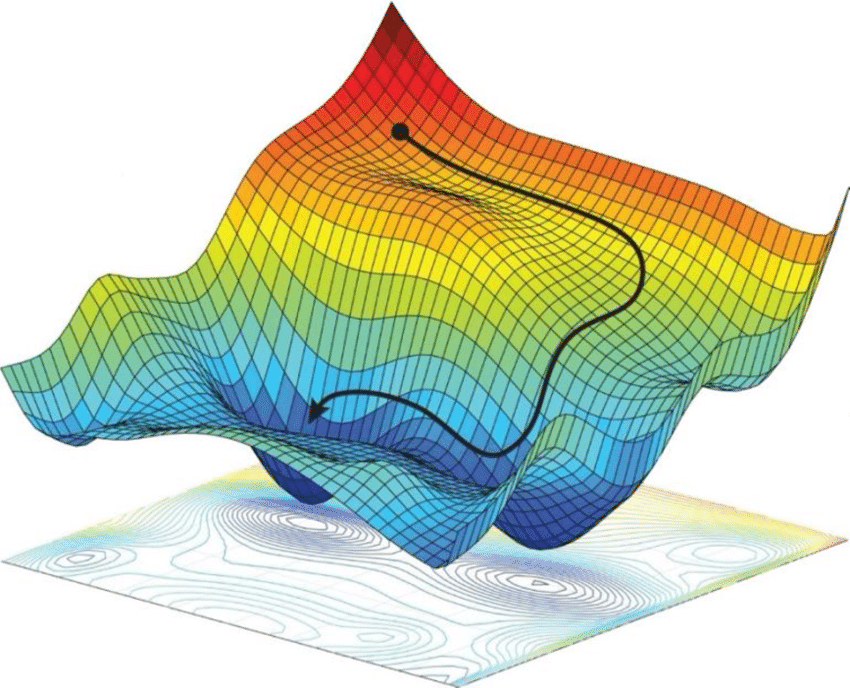
\includegraphics[scale=0.15]{Grad_Des_1.png}
        \caption{Descenso del gradiente}
    \end{figure}
\end{frame}

\begin{frame}{Optimizador Adam}
    Lo que un optimizador hace es mejorar los valores de los parámetros del módelo con el fin de reducir
    el error cometido por la red. El optimizador \textbf{Adam} es un optimizador adaptativo que surge de la combinación del
    adaptador \textbf{RMSProp} y \textbf{Momentum}.
    \begin{equation}
        \label{eqn:SRCNN_Adam}
        \begin{split}
            m&=\beta_1m+(1-\beta_1)\nabla W\\
            v&=\beta_2v+(1-\beta_2)\nabla W^2\\
            W&=W-\frac{\alpha m}{\sqrt{v+\epsilon}}
        \end{split}
    \end{equation}
\end{frame}

\begin{frame}{Error cuadrático medio}
    Mientras entrenamos el modelo, vamos a querer evaluar su precisión usando una función de costo (o pérdida), para ello podemos
    utilizar el error cuadrático medio, que se obtiene de la siguiente expresión:
    \begin{align}
        \label{eqn:SRCNN_MSE}
        MSE=\frac{1}{2m}\sum_{i=1}^{m}(\hat{y}_i-y_i)^2
    \end{align}
    \begin{figure}[H]
        \label{fig:SRCNN_MSE}
        \centering
        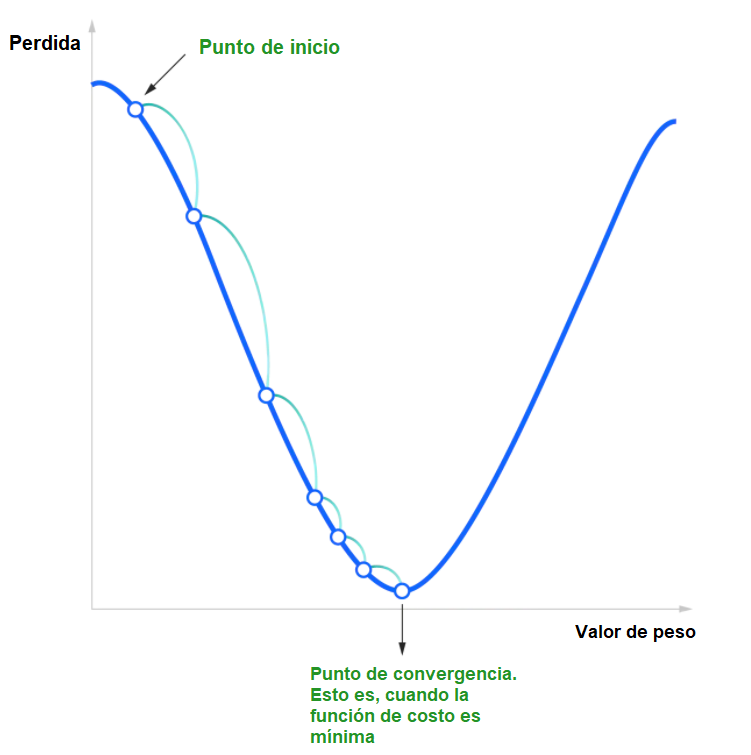
\includegraphics[width=5cm, height=3cm]{MSE.png}
        \caption{Minimización de función de costo}
    \end{figure}
\end{frame}

\begin{frame}{SRCNN}
    tradicionalmente se utilizan 3 etapas para la super resolución de imagenes, y estas se realizan por separado:
    \begin{enumerate}
        \item Extracción de parches en baja resolución y representación en un vector de gran dimensión
        \item Mapeo entre vectores (parches de baja resolución) de baja resolución con vectores que representan parches de alta
        resolución
        \item Reconstrucción de imagén
    \end{enumerate}
    \pause
    En \cite{SRCNN} proponen una red neuronal convolucional que realice estas 3 etapas en conjunto.
\end{frame}

\begin{frame}{SRCNN}
    La idea es tener una capa de entrada que se encargará de la extracción de características de baja resolución,
    una o más capas intermedias que se encargarán del mapeo entre características de baja resolución y las de alta resolución y
    una capa de salida que se encargará de la reconstrucción de la imagen de alta resolución.
    \begin{figure}[H]
        \label{fig:SRCNN_Arquitectura}
        \centering
        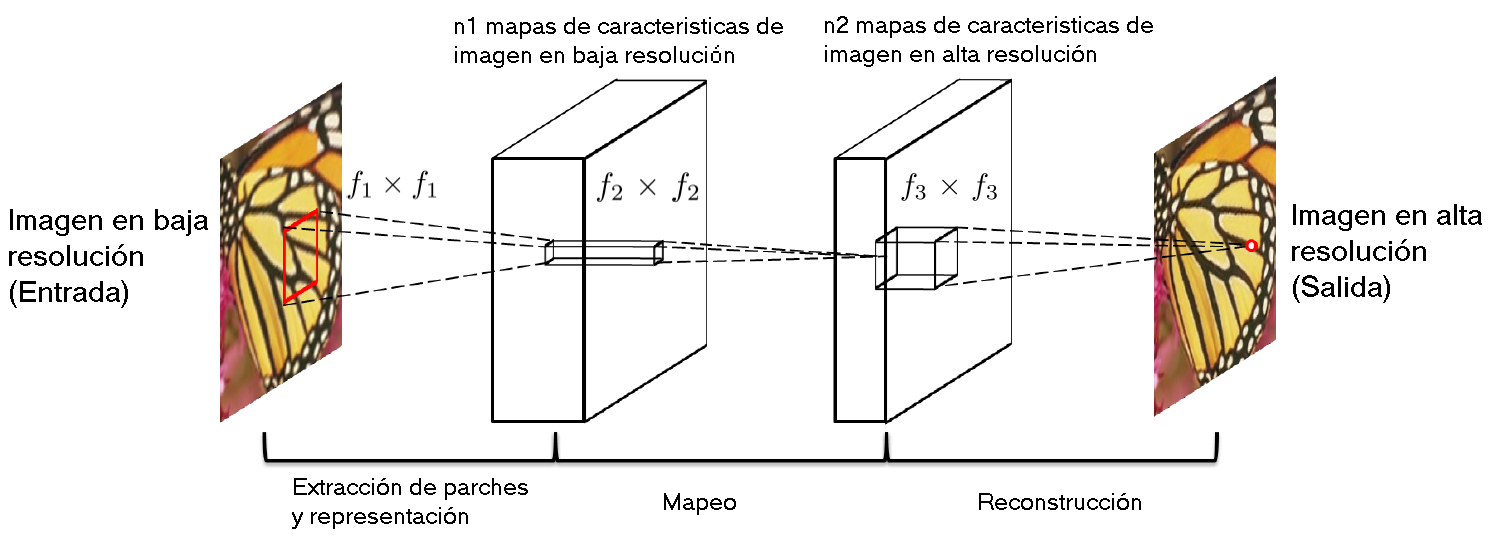
\includegraphics[scale = 0.3]{SRCNN_Arquitectura.png}
        \caption{Arquitectura de la SRCNN}
    \end{figure}
\end{frame}

\begin{frame}{SRCNN}
    Las operaciones que esta red realizará son las siguientes:\\
    \textbf{Capa 1}
    \begin{align}
        \label{eqn:SRCNN_FirstLayer}
        F_1(Y)=max(0,W_1*Y+B_1)
    \end{align}

    \textbf{Capa 2}
    \begin{align}
        \label{eqn:SRCNN_SecondLayer}
        F_2(Y)=max(0,W_2*F_1(Y)+B_2)
    \end{align}

    \textbf{Capa 3}
    \begin{align}
        \label{eqn:SRCNN_ThirdLayer}
        F(Y)=W_3*F_2(Y)+B_3
    \end{align}
\end{frame}